\documentclass[10pt]{beamer}

\usetheme{Madrid}
\usecolortheme{dolphin}
\usefonttheme{serif}

\usepackage[utf8]{inputenc}
\usepackage[T5]{fontenc}
\usepackage[vietnamese,english]{babel}
\usepackage{amsmath,amssymb}
\usepackage{array}
\usepackage{graphicx}
\usepackage{booktabs}
\usepackage{xcolor}
\usepackage{colortbl}
\usepackage{listings}
\definecolor{occupied}{RGB}{220,241,225}
\definecolor{epsiloncell}{RGB}{255,236,179}
\definecolor{checkcell}{RGB}{226,238,255}

\lstset{
    basicstyle=\ttfamily\scriptsize,
    columns=fullflexible,
    frame=single,
    breaklines=true
}

\title[Optimal Transport]{Optimal Transport}
\subtitle{Bài toán vận tải, bảng transportation, và Sinkhorn}
\author[Khánh \and Huy]{Nguyễn Quốc Khánh \and Nguyễn Xuân Huy}
\institute[UIT]{University of Information Technology -- VNU-HCM}
\date{May 2026}

\begin{document}

\begin{frame}
    \titlepage
\end{frame}

\begin{frame}{Roadmap}
    \begin{enumerate}
        \item \textbf{Giới thiệu:} OT là gì, vì sao nó giống bài toán vận tải.
        \item \textbf{Giải bảng transportation:} đọc bảng, tạo nghiệm ban đầu bằng Least Cost Method, rồi cải thiện bằng MODI/u-v.
        \item \textbf{Graph và thuật toán hiện đại:} nhìn bảng dưới dạng bipartite graph, dùng Python/POT, và giới thiệu Sinkhorn ở mức surface-level.
    \end{enumerate}
    \vspace{0.2cm}
    \centering
    Trọng tâm hôm nay: \textbf{discrete OT} với hữu hạn nguồn, đích, khối lượng và ma trận chi phí.
\end{frame}

\section{Giới thiệu}

\begin{frame}{Motivation}
    Nhiều đối tượng dữ liệu có thể nhìn như một phân phối khối lượng:
    ảnh, văn bản, embedding, hoặc dataset.

    \vspace{0.2cm}
    Khoảng cách vector thường so sánh từng vị trí:
    \[
        \text{vị trí }i\text{ của nguồn} \quad \text{với} \quad \text{vị trí }i\text{ của đích}.
    \]
    Nhưng nếu khối lượng chỉ ``dịch qua gần đó'', cách so sánh này có thể bỏ lỡ cấu trúc hình học.

    \vspace{0.2cm}
    Optimal Transport hỏi:
    \[
        \textit{Chi phí nhỏ nhất để chuyển phân phối này thành phân phối kia là bao nhiêu?}
    \]
    \[
        \text{OT cost}=\sum \text{khối lượng chuyển đi}\times \text{chi phí di chuyển}.
    \]
\end{frame}

\begin{frame}{Từ OT sang bài toán vận tải}
    Trong phiên bản rời rạc, ta có:
    \begin{itemize}
        \item các nguồn $S_i$ với supply $a_i$;
        \item các đích $D_j$ với demand $b_j$;
        \item chi phí vận chuyển một đơn vị từ $S_i$ đến $D_j$ là $C_{ij}$.
    \end{itemize}

    \[
        P_{ij}=\text{số lượng chuyển từ }S_i\text{ sang }D_j.
    \]

    Mục tiêu:
    \[
        \min_{P\ge 0}\sum_{i=1}^{m}\sum_{j=1}^{n} C_{ij}P_{ij}.
    \]

    Đây chính là dạng bảng quen thuộc của \textbf{Transportation Problem}.
\end{frame}

\begin{frame}{Điều kiện cân bằng}
    Một bảng transportation chuẩn thường giả sử:
    \[
        \sum_i a_i = \sum_j b_j.
    \]

    \begin{itemize}
        \item Tổng hàng có sẵn phải bằng tổng nhu cầu cần nhận.
        \item Nếu supply lớn hơn demand: thêm một đích giả (dummy destination).
        \item Nếu demand lớn hơn supply: thêm một nguồn giả (dummy source).
        \item Chi phí tới dummy thường đặt là $0$, vì phần này biểu diễn lượng dư hoặc thiếu giả định.
    \end{itemize}

    Trong ví dụ hôm nay, ta chọn bảng đã cân bằng để tập trung vào cách giải.
\end{frame}

\begin{frame}{Monge và Kantorovich:}
    \begin{columns}[T]
        \begin{column}{0.48\textwidth}
            \textbf{Monge}
            \[
                x \mapsto T(x)
            \]
            \begin{itemize}
                \item mỗi điểm nguồn chọn một điểm đích;
                \item trực quan nhưng khó xử lý;
                \item không tự nhiên khi cần chia nhỏ khối lượng.
            \end{itemize}
        \end{column}
        \begin{column}{0.48\textwidth}
            \textbf{Kantorovich}
            \[
                P_{ij}=\text{khối lượng từ }i\text{ sang }j
            \]
            \begin{itemize}
                \item cho phép mass splitting;
                \item đưa về ma trận;
                \item trở thành Linear Programming (LP) \cite{peyre2019computational}.
            \end{itemize}
        \end{column}
    \end{columns}
\end{frame}
\begin{frame}{Đọc điều kiện trên ma trận}
    \small
    Điều kiện của OT là:
    \[
        \sum_j P_{ij}=a_i,\qquad
        \sum_i P_{ij}=b_j,\qquad
        P_{ij}\ge 0.
    \]

    \vspace{0.1cm}
    Giả sử dữ liệu ban đầu có: $\mathbf{a} = (0.4, 0.3, 0.3)$ và $\mathbf{b} = (0.3, 0.4, 0.3)$.

    \vspace{0.2cm}
    \begin{columns}[T]
        \begin{column}{0.48\textwidth}
            Ví dụ một plan khả thi:
            \[
            P=
            \begin{pmatrix}
            \color{blue}{0.1}&\color{blue}{0.2}&\color{blue}{0.1}\\
            0.1&0.1&0.1\\
            0.1&0.1&0.1
            \end{pmatrix}
            \]
        \end{column}
        \begin{column}{0.48\textwidth}
            Hàng 1 là tổng lượng rời khỏi $S_1$:
            \[
                0.1+0.2+0.1 = a_1 = 0.4.
            \]
            Cột 2 là tổng lượng đi vào $D_2$:
            \[
                0.2+0.1+0.1 = b_2 = 0.4.
            \]
        \end{column}
    \end{columns}
\end{frame}

\section{Giải bảng transportation}

\begin{frame}{Các nhóm phương pháp giải bảng}
    Trong Operations Research, bài toán vận tải thường được giải theo hai pha.

    \vspace{0.15cm}
    \textbf{Pha 1: tìm nghiệm cơ sở khả thi ban đầu}
    \begin{itemize}
        \item Northwest Corner Method;
        \item Least Cost Method;
        \item Vogel's Approximation Method (VAM).
    \end{itemize}

    \textbf{Pha 2: kiểm tra và cải thiện tối ưu}
    \begin{itemize}
        \item Stepping Stone;
        \item MODI/u-v method;
        \item transportation simplex.
    \end{itemize}

    Hôm nay ta dùng \textbf{Least Cost Method + MODI/u-v}: đủ trực quan nhưng vẫn có tính toán thật.
\end{frame}

\begin{frame}{Ví dụ bảng transportation}
    \[
    C=
    \begin{pmatrix}
    8&11&10\\
    2&10&1\\
    15&14&8
    \end{pmatrix},
    \qquad
    a=(17,28,27),\quad b=(16,24,32).
    \]

    \begin{center}
    \begin{tabular}{c|ccc|c}
        \toprule
        & $D_1$ & $D_2$ & $D_3$ & Supply\\
        \midrule
        $S_1$ & 8 & 11 & 10 & 17\\
        $S_2$ & 2 & 10 & 1 & 28\\
        $S_3$ & 15 & 14 & 8 & 27\\
        \midrule
        Demand & 16 & 24 & 32 & 72\\
        \bottomrule
    \end{tabular}
    \end{center}

    Bài toán cân bằng vì tổng supply $=72=$ tổng demand.
\end{frame}

\begin{frame}{Least Cost Method: Ý tưởng}
    \small
    Least Cost Method (LCM) là một heuristic để tạo nghiệm ban đầu (Initial Basic Feasible Solution).

    \begin{block}{Dữ liệu bài toán (Input \& Output)}
        \begin{itemize}
            \item \textbf{Input:} Ma trận chi phí $C \in \mathbb{R}^{m \times n}_+$, vectơ cung $a=(a_1,\dots,a_m)$ và vectơ cầu $b=(b_1,\dots,b_n)$.
            \item \textbf{Output:} Ma trận phân bổ hàng hóa $P \in \mathbb{R}^{m \times n}_+$, khởi tạo $P_{ij}=0$.
        \end{itemize}
    \end{block}

    \begin{enumerate}
        \item Chọn ô chưa bị gạch bỏ có chi phí đơn vị nhỏ nhất $C_{ij}$.
        \item Gán lượng hàng nhiều nhất có thể:
        \[
            P_{ij}=\min\left(a_i^{(t)}, b_j^{(t)}\right).
        \]
        \item Cập nhật supply/demand còn lại:
        \[
            a_i^{(t+1)}=a_i^{(t)}-P_{ij},\quad
            b_j^{(t+1)}=b_j^{(t)}-P_{ij}.
        \]
        \item Gạch bỏ hàng $i$ nếu $a_i^{(t+1)}=0$ hoặc cột $j$ nếu $b_j^{(t+1)}=0$, rồi lặp lại từ Bước 1.
    \end{enumerate}

    \vskip 0.1cm
    \textit{Lưu ý:} LCM luôn chọn tuyến rẻ nhất trước, nhưng \textbf{chưa đảm bảo tối ưu toàn cục} do bản chất greedy cục bộ.
\end{frame}

\begin{frame}{LCM: các bước gán}
    \scriptsize
    \begin{columns}[T]
        \begin{column}{0.36\textwidth}
            \centering
            \textbf{Bảng chi phí}
            \vspace{0.05cm}

            \resizebox{\textwidth}{!}{%
            \begin{tabular}{c|ccc|c}
                \toprule
                & $D_1$ & $D_2$ & $D_3$ & Supply\\
                \midrule
                $S_1$ & 8 & 11 & 10 & 17\\
                $S_2$ & 2 & 10 & 1 & 28\\
                $S_3$ & 15 & 14 & 8 & 27\\
                \midrule
                Demand & 16 & 24 & 32 & 72\\
                \bottomrule
            \end{tabular}}
        \end{column}
        \begin{column}{0.62\textwidth}
            \centering
            \textbf{Các bước gán theo LCM}
            \vspace{0.05cm}

            \resizebox{\textwidth}{!}{%
            \begin{tabular}{c|c|c|c}
                \toprule
                Bước & Ô chọn & Lượng gán & Lý do\\
                \midrule
                1 & $(S_2,D_3)$ & 28 & chi phí nhỏ nhất $1$\\
                2 & $(S_1,D_1)$ & 16 & chi phí nhỏ nhất còn lại $8$\\
                3 & $(S_3,D_3)$ & 4 & $D_3$ còn thiếu $4$\\
                4 & $(S_1,D_2)$ & 1 & $S_1$ còn $1$\\
                5 & $(S_3,D_2)$ & 23 & phần còn lại của $D_2$\\
                \bottomrule
            \end{tabular}}
        \end{column}
    \end{columns}

    \vspace{0.15cm}
    \[
    P_0=
    \begin{pmatrix}
    16&1&0\\
    0&0&28\\
    0&23&4
    \end{pmatrix}
    \]
\end{frame}

\begin{frame}{LCM: tính cost ban đầu}
    \[
    P_0=
    \begin{pmatrix}
    16&1&0\\
    0&0&28\\
    0&23&4
    \end{pmatrix}
    \]

    \[
    \begin{aligned}
    \langle P_0,C\rangle
    &=16\cdot 8+1\cdot 11+28\cdot 1+23\cdot 14+4\cdot 8\\
    &=128+11+28+322+32\\
    &=521.
    \end{aligned}
    \]

    Câu hỏi tiếp theo: nghiệm này đã tối ưu chưa?
\end{frame}

\begin{frame}{MODI/u-v: ý tưởng}
    MODI/u-v method kiểm tra xem có ô trống nào đáng đưa hàng vào hay không.

    \begin{itemize}
        \item Với các ô đang dùng, tìm $u_i,v_j$ sao cho
        \[
            u_i+v_j=C_{ij}.
        \]
        \item Với ô trống, tính reduced cost:
        \[
            \Delta_{ij}=C_{ij}-(u_i+v_j).
        \]
        \item Nếu có $\Delta_{ij}<0$, đưa hàng vào ô đó có thể giảm tổng chi phí.
        \item Nếu mọi $\Delta_{ij}\ge 0$, nghiệm hiện tại là tối ưu.
    \end{itemize}
\end{frame}

\begin{frame}{MODI: tính potentials}
    Với $P_0$, các ô đang dùng là:
    \[
        (1,1),(1,2),(2,3),(3,2),(3,3).
    \]
    Đặt $u_1=0$, giải hệ $u_i+v_j=C_{ij}$ trên các ô này:
    \[
        u=(0,-4,3),\qquad v=(8,11,5).
    \]

    Khi đó reduced cost của các ô trống:
    \[
    \begin{array}{c|ccc}
        & D_1&D_2&D_3\\
        \hline
        S_1&0&0&5\\
        S_2&\color{red}{-2}&3&0\\
        S_3&4&0&0
    \end{array}
    \]

    Ô $(S_2,D_1)$ có $\Delta_{21}=-2$, nên ta cải thiện theo ô này.
\end{frame}

\begin{frame}{MODI: vòng điều chỉnh}
    Bắt đầu từ ô mới $(S_2,D_1)$, tạo vòng kín qua các ô đang dùng:
    \[
    (2,1)^+ \to (2,3)^- \to (3,3)^+ \to (3,2)^-
    \to (1,2)^+ \to (1,1)^-.
    \]

    Chọn
    \[
        \theta=\min\{P_{23},P_{32},P_{11}\}
        =\min\{28,23,16\}=16.
    \]

    Cộng $\theta$ vào dấu $+$ và trừ $\theta$ khỏi dấu $-$.
    Đây là cách dịch hàng mà vẫn giữ đúng tổng supply và demand.
\end{frame}

\begin{frame}{Kết quả sau một lần cải thiện}
    \[
    P^\star=
    \begin{pmatrix}
    0&17&0\\
    16&0&12\\
    0&7&20
    \end{pmatrix}
    \]

    \[
    \begin{aligned}
    \langle P^\star,C\rangle
    &=17\cdot 11+16\cdot 2+12\cdot 1+7\cdot 14+20\cdot 8\\
    &=187+32+12+98+160\\
    &=489.
    \end{aligned}
    \]

\end{frame}

\begin{frame}{Kiểm tra tối ưu sau MODI}
    Với $P^\star$, đặt lại $u_1=0$ và giải trên các ô đang dùng:
    \[
        u=(0,-4,3),\qquad v=(6,11,5).
    \]

    Reduced cost của các ô trống:
    \[
    \begin{array}{c|ccc}
        & D_1&D_2&D_3\\
        \hline
        S_1&2&0&5\\
        S_2&0&3&0\\
        S_3&6&0&0
    \end{array}
    \]

    Tất cả reduced cost đều không âm, nên không có ô trống nào giúp giảm chi phí nữa.
    Đây là tiêu chuẩn dừng của MODI.
    Sau khi kiểm tra lại MODI, không còn reduced cost âm, nên nghiệm này tối ưu.
    \vspace{0.15cm}
    Ở bài này, số ô cơ sở là $5=m+n-1$, nên MODI chạy bình thường.
    Bài tiếp theo sẽ cho thấy điều gì xảy ra khi số ô cơ sở bị thiếu.
\end{frame}
\section{Bài toán 2: Bảng chữ nhật + suy biến}

\begin{frame}{Từ Bài toán 1 sang Bài toán 2}
    \begin{columns}[T]
        \begin{column}{0.48\textwidth}
            \textbf{Bài toán 1: normal case}
            \begin{itemize}
                \item Bảng $3\times 3$.
                \item Least Cost tạo một cơ sở khả thi.
                \item MODI phát hiện $\Delta_{21}<0$, cải thiện, rồi dừng.
                \item Đủ ô cơ sở: $5=m+n-1$.
            \end{itemize}
        \end{column}
        \begin{column}{0.48\textwidth}
            \textbf{Bài toán 2: degenerate case}
            \begin{itemize}
                \item Bảng $3\times 4$.
                \item Least Cost result đã tối ưu.
                \item Nhưng chỉ có $5<m+n-1=6$ ô cơ sở.
                \item Cần $\varepsilon$ trước khi MODI verify.
            \end{itemize}
        \end{column}
    \end{columns}

    \vspace{0.25cm}
    \begin{block}{Nhịp trình bày}
        Cùng Least Cost + MODI, nhưng Problem 2 tập trung vào degeneracy.
    \end{block}
\end{frame}
\note{Gợi ý viết bảng: kẻ một đường dọc. Bên trái ghi ``Bài 1: MODI bình thường''. Bên phải ghi ``Bài 2: vẫn là MODI, nhưng cơ sở thiếu 1 ô''. Như vậy người nghe thấy rõ ví dụ này không chỉ là lặp lại.}

\begin{frame}{Bài toán 2: Bảng chữ nhật + suy biến}
    Ta bỏ qua phần tính Least Cost chi tiết và bắt đầu từ kết quả của nó.

    \vspace{0.3cm}
    \begin{block}{Mục tiêu}
        Kiểm tra một transportation problem cân bằng $3 \times 4$ bằng MODI, kể cả khi cơ sở ban đầu bị suy biến.
    \end{block}

    \vspace{0.1cm}
    \centering
    \renewcommand{\arraystretch}{1.15}
    \begin{tabular}{c|cccc|c}
        & $D_1$ & $D_2$ & $D_3$ & $D_4$ & Cung\\
        \hline
        $S_1$ & $1$ & $8$ & $9$ & $6$ & $20$\\
        $S_2$ & $7$ & $2$ & $8$ & $3$ & $30$\\
        $S_3$ & $7$ & $8$ & $5$ & $4$ & $25$\\
        \hline
        Cầu & $20$ & $25$ & $20$ & $10$ & $75$
    \end{tabular}

    \vspace{0.12cm}
    \[
        C =
        \begin{pmatrix}
            1 & 8 & 9 & 6\\
            7 & 2 & 8 & 3\\
            7 & 8 & 5 & 4
        \end{pmatrix},
        \qquad
        s=(20,30,25),\quad d=(20,25,20,10)
    \]
    \vspace{-0.1cm}
    \[
        \sum_i s_i = 75 = \sum_j d_j.
    \]
\end{frame}
\note{Gợi ý viết bảng: ghi ``Bài toán 2'' cùng ba số $m=3$, $n=4$, $m+n-1=6$. Nhắc rằng phần Least Cost đã được giả sử xong, nên bảng chỉ dùng cho MODI.}

\begin{frame}{Kết quả Least Cost: đếm số ô cơ sở}
    \centering
    \renewcommand{\arraystretch}{1.25}
    \begin{tabular}{c|cccc|c}
        & $D_1$ & $D_2$ & $D_3$ & $D_4$ & Supply\\
        \hline
        $S_1$ & \cellcolor{occupied}$20$ {\scriptsize $(1)$} & {\scriptsize $(8)$} & {\scriptsize $(9)$} & {\scriptsize $(6)$} & $20$\\
        $S_2$ & {\scriptsize $(7)$} & \cellcolor{occupied}$25$ {\scriptsize $(2)$} & {\scriptsize $(8)$} & \cellcolor{occupied}$5$ {\scriptsize $(3)$} & $30$\\
        $S_3$ & {\scriptsize $(7)$} & {\scriptsize $(8)$} & \cellcolor{occupied}$20$ {\scriptsize $(5)$} & \cellcolor{occupied}$5$ {\scriptsize $(4)$} & $25$\\
        \hline
        Demand & $20$ & $25$ & $20$ & $10$ &
    \end{tabular}

    \vspace{0.35cm}
    \begin{columns}[T]
        \begin{column}{0.48\textwidth}
            \[
                \#\text{ ô cơ sở}=5
            \]
        \end{column}
        \begin{column}{0.48\textwidth}
            \[
                m+n-1=3+4-1=6
            \]
        \end{column}
    \end{columns}

    \vspace{0.15cm}
    \begin{alertblock}{Kết luận}
        Đây là một phương án cơ sở khả thi bị suy biến.
    \end{alertblock}
\end{frame}
\note{Gợi ý viết bảng: ghi $B=\{(1,1),(2,2),(2,4),(3,3),(3,4)\}$, rồi $|B|=5<6$. Chỉ vào năm ô xanh khi đọc tên từng ô.}

\begin{frame}{Vì sao suy biến gây vấn đề}
    MODI gán thế vị hàng và cột dựa trên các ô cơ sở:
    \[
        c_{ij}=u_i+v_j.
    \]

    \vspace{0.2cm}
    \begin{itemize}
        \item Bài toán $3 \times 4$ có $3+4=7$ thế vị.
        \item Chọn một thế vị, ví dụ $u_1=0$, thì còn $6$ giá trị chưa biết.
        \item Vì vậy ta cần $m+n-1=6$ ô cơ sở để có đủ phương trình.
    \end{itemize}

    \vspace{0.2cm}
    \begin{block}{Trực giác}
        Chỉ có $5$ ô cơ sở thì các phương trình MODI chưa nối được toàn bộ bảng.
    \end{block}
\end{frame}
\note{Gợi ý viết bảng: vẽ basis graph với các nút hàng $S_i$ và nút cột $D_j$. Cho thấy $S_1-D_1$ bị tách khỏi các ô cơ sở còn lại, nên phương trình thế vị không lan ra được toàn bảng.}

\begin{frame}{Sửa suy biến bằng epsilon}
    Thêm một lượng hàng tượng trưng bằng $0$ vào một ô trống:
    \[
        x_{14}=\varepsilon.
    \]

    \centering
    \renewcommand{\arraystretch}{1.25}
    \begin{tabular}{c|cccc|c}
        & $D_1$ & $D_2$ & $D_3$ & $D_4$ & Cung\\
        \hline
        $S_1$ & \cellcolor{occupied}$20$ & & & \cellcolor{epsiloncell}$\varepsilon$ & $20$\\
        $S_2$ & & \cellcolor{occupied}$25$ & & \cellcolor{occupied}$5$ & $30$\\
        $S_3$ & & & \cellcolor{occupied}$20$ & \cellcolor{occupied}$5$ & $25$\\
        \hline
        Cầu & $20$ & $25$ & $20$ & $10$ &
    \end{tabular}

    \vspace{0.25cm}
    \begin{itemize}
        \item $\varepsilon$ được tính như một ô cơ sở trong MODI.
        \item Nó là zero shipment, nên lượng hàng và chi phí không đổi.
    \end{itemize}
\end{frame}
\note{Gợi ý viết bảng: thêm cạnh $(1,4)$ vào basis graph. Nói vì sao ô này tiện: nó nối phần cô lập $S_1-D_1$ với phần chứa $D_4$ và không tạo cycle.}

\begin{frame}{Các phương trình MODI từ cơ sở}
    \begin{columns}[c]
        \begin{column}{0.58\textwidth}
            Với mỗi ô cơ sở, kể cả ô $\varepsilon$, viết
            \[
                c_{ij}=u_i+v_j,
                \qquad u_1=0.
            \]

            \vspace{-0.15cm}
            \[
            \begin{aligned}
                S_1D_1 &: u_1+v_1=1,\\
                S_1D_4 &: u_1+v_4=6,\\
                S_2D_2 &: u_2+v_2=2,\\
                S_2D_4 &: u_2+v_4=3,\\
                S_3D_3 &: u_3+v_3=5,\\
                S_3D_4 &: u_3+v_4=4.
            \end{aligned}
            \]
        \end{column}
        \begin{column}{0.36\textwidth}
            \centering
            \scriptsize
            \textbf{Bảng chi phí}\\[0.08cm]
            \renewcommand{\arraystretch}{1.2}
            \begin{tabular}{c|cccc}
                & $D_1$ & $D_2$ & $D_3$ & $D_4$\\
                \hline
                $S_1$ & \cellcolor{occupied}$1$ & $8$ & $9$ & \cellcolor{epsiloncell}$6$\\
                $S_2$ & $7$ & \cellcolor{occupied}$2$ & $8$ & \cellcolor{occupied}$3$\\
                $S_3$ & $7$ & $8$ & \cellcolor{occupied}$5$ & \cellcolor{occupied}$4$
            \end{tabular}
        \end{column}
    \end{columns}

    \vspace{0.05cm}
    \begin{block}{Ý chính}
        Ô $\varepsilon$ tạo phương trình còn thiếu: $u_1+v_4=6$.
    \end{block}
\end{frame}
\note{Gợi ý viết bảng: viết sáu phương trình thành hai cột. Khoanh $u_1=0$ và phương trình epsilon $u_1+v_4=6$, vì đây là cầu nối giúp giải được phần còn lại.}

\begin{frame}{Giải các thế vị}
    \begin{columns}[c]
        \begin{column}{0.58\textwidth}
            Bắt đầu với $u_1=0$, rồi đi theo các ô cơ sở đã nối:
            \[
            \begin{aligned}
                u_1+v_1=1 &\Rightarrow v_1=1,\\
                u_1+v_4=6 &\Rightarrow v_4=6,\\
                u_2+v_4=3 &\Rightarrow u_2=-3,\\
                u_2+v_2=2 &\Rightarrow v_2=5,\\
                u_3+v_4=4 &\Rightarrow u_3=-2,\\
                u_3+v_3=5 &\Rightarrow v_3=7.
            \end{aligned}
            \]
        \end{column}
        \begin{column}{0.36\textwidth}
            \centering
            \scriptsize
            \textbf{Bảng chi phí}\\[0.08cm]
            \renewcommand{\arraystretch}{1.2}
            \begin{tabular}{c|cccc}
                & $D_1$ & $D_2$ & $D_3$ & $D_4$\\
                \hline
                $S_1$ & \cellcolor{occupied}$1$ & $8$ & $9$ & \cellcolor{epsiloncell}$6$\\
                $S_2$ & $7$ & \cellcolor{occupied}$2$ & $8$ & \cellcolor{occupied}$3$\\
                $S_3$ & $7$ & $8$ & \cellcolor{occupied}$5$ & \cellcolor{occupied}$4$
            \end{tabular}
        \end{column}
    \end{columns}

    \vspace{0.1cm}
    \begin{center}
        \renewcommand{\arraystretch}{1.2}
        \begin{tabular}{rl}
            \textbf{Hàng:} &
            $u_1=0,\quad u_2=-3,\quad u_3=-2$\\
            \textbf{Cột:} &
            $v_1=1,\quad v_2=5,\quad v_3=7,\quad v_4=6$
        \end{tabular}
    \end{center}
\end{frame}
\note{Gợi ý viết bảng: giải đúng theo thứ tự này bằng mũi tên. Câu chuyện gọn là: $u_1$ cho $v_1$ và $v_4$; $v_4$ cho $u_2$ và $u_3$; rồi $u_2$ cho $v_2$, $u_3$ cho $v_3$.}

\begin{frame}{Kiểm tra chi phí cơ hội}
    Với mỗi ô trống, tính reduced cost:
    \[
        \Delta_{ij}=c_{ij}-(u_i+v_j).
    \]

    \vspace{-0.1cm}
    \begin{columns}[c]
        \begin{column}{0.58\textwidth}
            \[
            \begin{aligned}
                \Delta_{12}&=8-(0+5)=3,\\
                \Delta_{13}&=9-(0+7)=2,\\
                \Delta_{21}&=7-(-3+1)=9,\\
                \Delta_{23}&=8-(-3+7)=4,\\
                \Delta_{31}&=7-(-2+1)=8,\\
                \Delta_{32}&=8-(-2+5)=5.
            \end{aligned}
            \]
        \end{column}
        \begin{column}{0.36\textwidth}
            \centering
            \scriptsize
            \textbf{Bảng chi phí}\\[0.08cm]
            \renewcommand{\arraystretch}{1.2}
            \begin{tabular}{c|cccc}
                & $D_1$ & $D_2$ & $D_3$ & $D_4$\\
                \hline
                $S_1$ & \cellcolor{occupied}$1$ & \cellcolor{checkcell}$8$ & \cellcolor{checkcell}$9$ & \cellcolor{epsiloncell}$6$\\
                $S_2$ & \cellcolor{checkcell}$7$ & \cellcolor{occupied}$2$ & \cellcolor{checkcell}$8$ & \cellcolor{occupied}$3$\\
                $S_3$ & \cellcolor{checkcell}$7$ & \cellcolor{checkcell}$8$ & \cellcolor{occupied}$5$ & \cellcolor{occupied}$4$
            \end{tabular}
        \end{column}
    \end{columns}

    \vspace{0.05cm}
    \begin{alertblock}{Quyết định MODI}
        Mọi ô trống đều có $\Delta_{ij}>0$, nên không có ô vào nào giúp giảm chi phí.
    \end{alertblock}
\end{frame}
\note{Gợi ý viết bảng: tính chậm một ví dụ, chẳng hạn $\Delta_{12}=8-(0+5)=3$. Sau đó điền nhanh năm giá trị còn lại như checklist. Vì reduced cost nhỏ nhất vẫn dương, dừng.}

\begin{frame}{Kết luận chính}
    \begin{itemize}
        \item Suy biến không có nghĩa là phương án sai hoặc không khả thi.
        \item Nó chỉ có nghĩa là MODI cần một ô cơ sở tượng trưng để tiếp tục.
        \item Sau khi thêm $\varepsilon$, các reduced cost chứng minh phương án tối ưu.
    \end{itemize}

    \vspace{0.3cm}
    \begin{block}{Chi phí cuối cùng}
        \[
            20(1)+25(2)+5(3)+20(5)+5(4)=\mathbf{205}.
        \]
    \end{block}
\end{frame}
\note{Gợi ý viết bảng: ghi ``Suy biến $\neq$ sai'' và gạch dưới chi phí cuối cùng $205$. Nhắc rằng $\varepsilon$ không tính vào chi phí vì nó là zero shipment.}

\begin{frame}[fragile]{Kiểm chứng bằng exact LP: POT}
    \begin{columns}[c]
        \begin{column}{0.44\textwidth}
            Exact OT solver của POT trả về
            \[
                P_{\text{POT}}=
                \begin{pmatrix}
                    20 & 0 & 0 & 0\\
                    0 & 25 & 0 & 5\\
                    0 & 0 & 20 & 5
                \end{pmatrix}.
            \]

            \[
                \langle P_{\text{POT}}, C\rangle = 205.
            \]

            \begin{block}{Khớp với MODI}
                Cùng pattern vận chuyển và chi phí.
            \end{block}

            {\scriptsize Ghi chú: $\langle P,C\rangle=\sum_{i,j}P_{ij}C_{ij}$ là nhân từng phần tử rồi cộng lại.}
        \end{column}
        \begin{column}{0.52\textwidth}
            \textbf{Code}
            \begin{lstlisting}[language=Python,basicstyle=\ttfamily\tiny]
import numpy as np
import ot

s = np.array([20, 30, 25.])
d = np.array([20, 25, 20, 10.])
C = np.array([[1, 8, 9, 6],
              [7, 2, 8, 3],
              [7, 8, 5, 4]], float)

P = ot.emd(s, d, C)
print(P.astype(int))
print((P * C).sum())
            \end{lstlisting}
            \textbf{Output}
            \begin{lstlisting}[basicstyle=\ttfamily\tiny]
[[20  0  0  0]
 [ 0 25  0  5]
 [ 0  0 20  5]]
205.0
            \end{lstlisting}
        \end{column}
    \end{columns}
\end{frame}
\note{Đây là slide kiểm chứng dự phòng. Nếu thiếu thời gian, chỉ nói miệng: POT ot.emd và SciPy linprog đều trả về cùng phương án này với objective 205.}

\section{Graph và thuật toán hiện đại}

\begin{frame}{Nhìn bảng dưới dạng bipartite graph}
    \textbf{Bipartite graph:} hai nhóm node, cạnh chỉ nối từ nhóm trái sang nhóm phải.

    \[
        \{S_1,S_2,S_3,\dots,S_m\}
        \quad\longrightarrow\quad
        \{D_1,D_2,D_3,\dots,D_n\}
    \]

    \begin{itemize}
        \item mỗi ô trong bảng là một cạnh $S_i\to D_j$;
        \item cost của cạnh là $C_{ij}$;
        \item flow trên cạnh là $P_{ij}$;
        \item trong mô hình OT cơ bản, cạnh giữa $S_i$ và $D_j$ không cần capacity riêng; giới hạn đến từ supply và demand.
    \end{itemize}

    Đây là cách nhìn transportation problem như một min-cost flow đặc biệt \cite{dong2020study}.
\end{frame}

\begin{frame}{Visualization của bipartite graph}
    \centering
    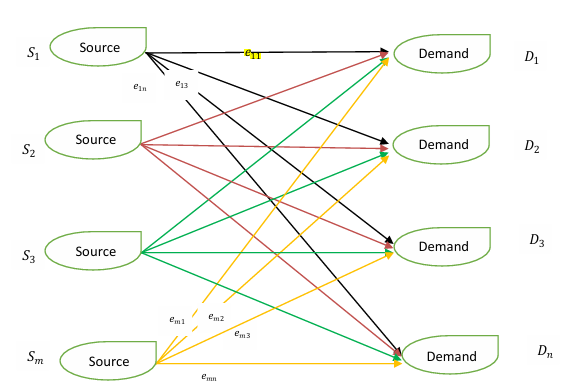
\includegraphics[width=0.8\textwidth]{Untitled.png}

    \vspace{0.15cm}
    Mỗi đường nối biểu diễn một tuyến vận chuyển có chi phí riêng.
\end{frame}

\begin{frame}{Exact solvers ở mức high-level}
    Cách giải bảng bằng MODI là phiên bản thủ công, phù hợp cho ví dụ nhỏ.

    \vspace{0.15cm}
    Với dữ liệu lớn hơn, exact solver thường dùng:
    \begin{itemize}
        \item transportation simplex / network simplex;
        \item min-cost flow algorithms;
        \item LP solvers.
    \end{itemize}

    % Ý tưởng chung: tìm một kế hoạch vận chuyển hợp lệ, rồi cải thiện dần cho đến khi không còn cách giảm chi phí.
\end{frame}

% \begin{frame}{Vì sao cần phương pháp hiện đại?}
%     Với histogram có $d$ vị trí và ground metric tổng quát, Cuturi dùng mốc
%     \[
%         O(d^3\log d)
%     \]
%     như động lực tính toán cho Sinkhorn \cite{cuturi2013sinkhorn}.

%     \begin{itemize}
%         \item Ở đây $d$ là số vị trí/hỗ trợ của histogram.
%         \item Nếu hai phân phối đều có $n$ điểm, có thể đọc gần như $O(n^3\log n)$.
%         \item Với ML, ta có thể phải tính OT rất nhiều lần trong training loop.
%     \end{itemize}

%     Vì vậy exact OT tốt cho bài nhỏ, nhưng có thể nặng khi dữ liệu lớn.
% \end{frame}

\begin{frame}[fragile]{Dùng Python Optimal Transport (POT)}
    POT cho phép gọi exact OT và Sinkhorn trực tiếp \cite{flamary2021pot}.

\begin{lstlisting}[language=Python]
import ot

C = ot.dist(X, Y, metric="sqeuclidean")

P_exact = ot.emd(a, b, C)
P_sinkhorn = ot.sinkhorn(a, b, C, reg=0.06)
\end{lstlisting}

    \begin{itemize}
        \item \texttt{ot.emd}: exact discrete OT.
        \item \texttt{ot.sinkhorn}: xấp xỉ có entropic regularization.
    \end{itemize}
\end{frame}

\begin{frame}{Sinkhorn: exact plan vs soft plan}
    \small
    Sinkhorn thêm entropy để tạo một transport plan mềm hơn và dễ tính hơn \cite{cuturi2013sinkhorn}.

    \vspace{0.08cm}
    \centering
    \IfFileExists{pot_transport_edges.png}{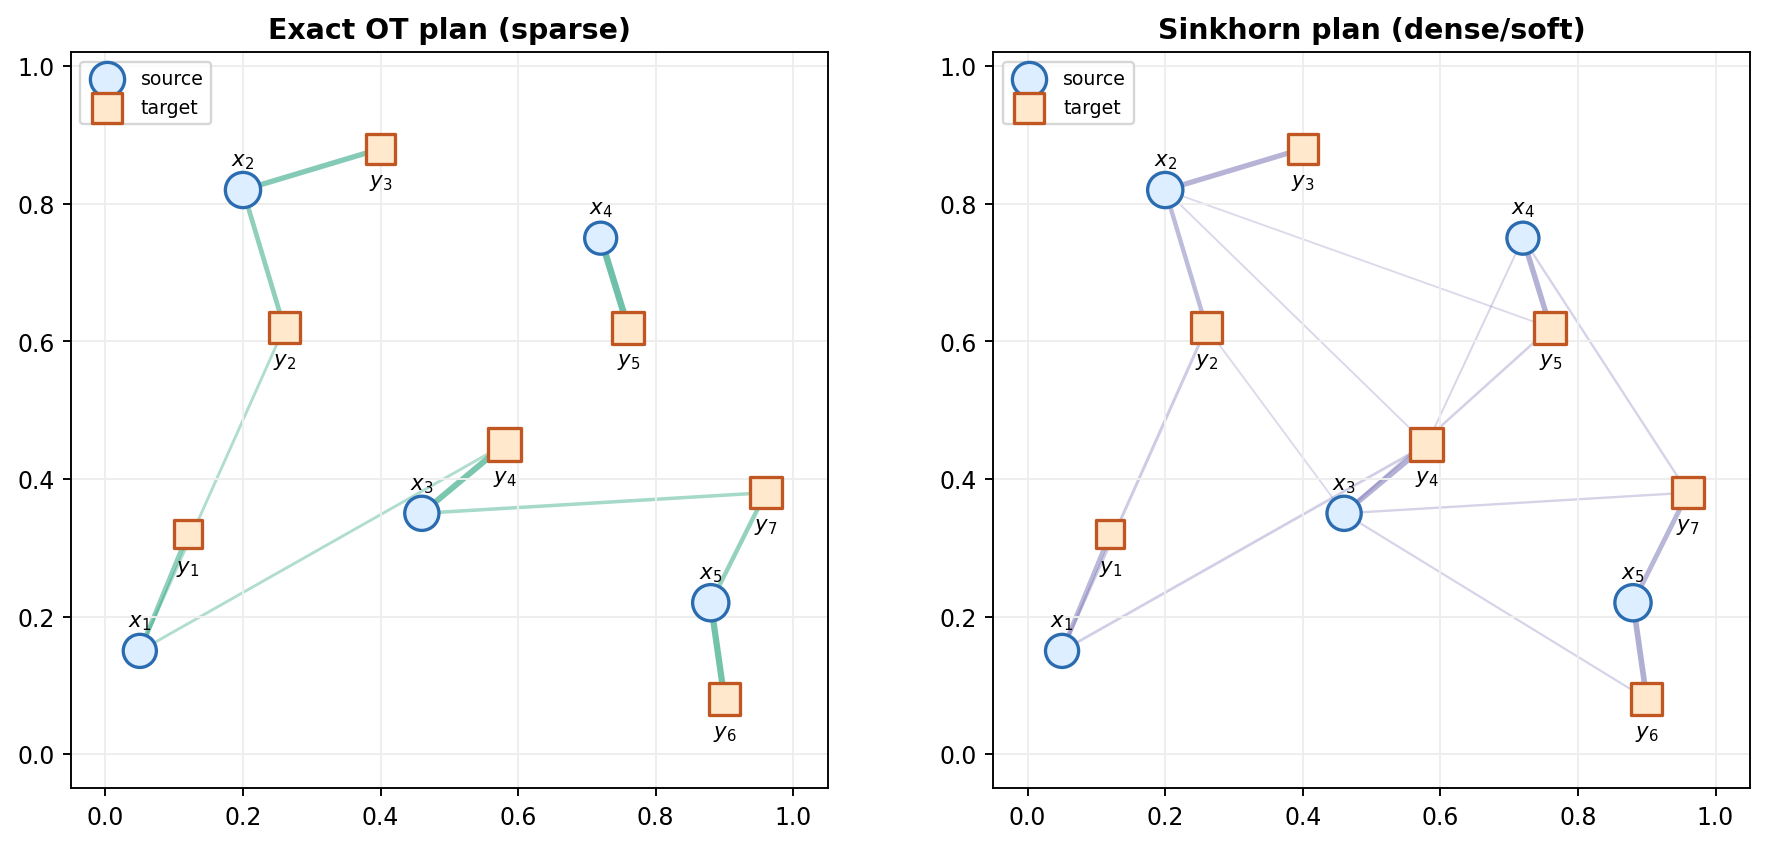
\includegraphics[width=0.76\textwidth]{pot_transport_edges.png}}{\fbox{\parbox{0.76\textwidth}{\centering Exact plan vs Sinkhorn plan}}}

    \vspace{0.08cm}
    \begin{itemize}
        \item Exact OT: sparse/hard, nhiều ô bằng $0$.
        \item Sinkhorn: dense/soft, khối lượng trải ra nhiều tuyến hơn.
        \item Dùng nhiều trong ML vì tính toán mượt hơn cho gradient-based learning.
    \end{itemize}
\end{frame}

\begin{frame}{Ứng dụng hiện đại}
    \small
    \begin{itemize}
        \item \textbf{NLP:} Word Mover's Distance so sánh văn bản qua word embeddings \cite{kusner2015word}.
        \item \textbf{Generative models:} dùng Wasserstein/Sinkhorn losses để so sánh phân phối dữ liệu sinh ra và dữ liệu thật \cite{cuturi2013sinkhorn,peyre2019computational}.
        \item \textbf{Domain adaptation:} dữ liệu cũ có label, dữ liệu mới chưa có label.
    \end{itemize}

    \vspace{0.05cm}
    \centering
    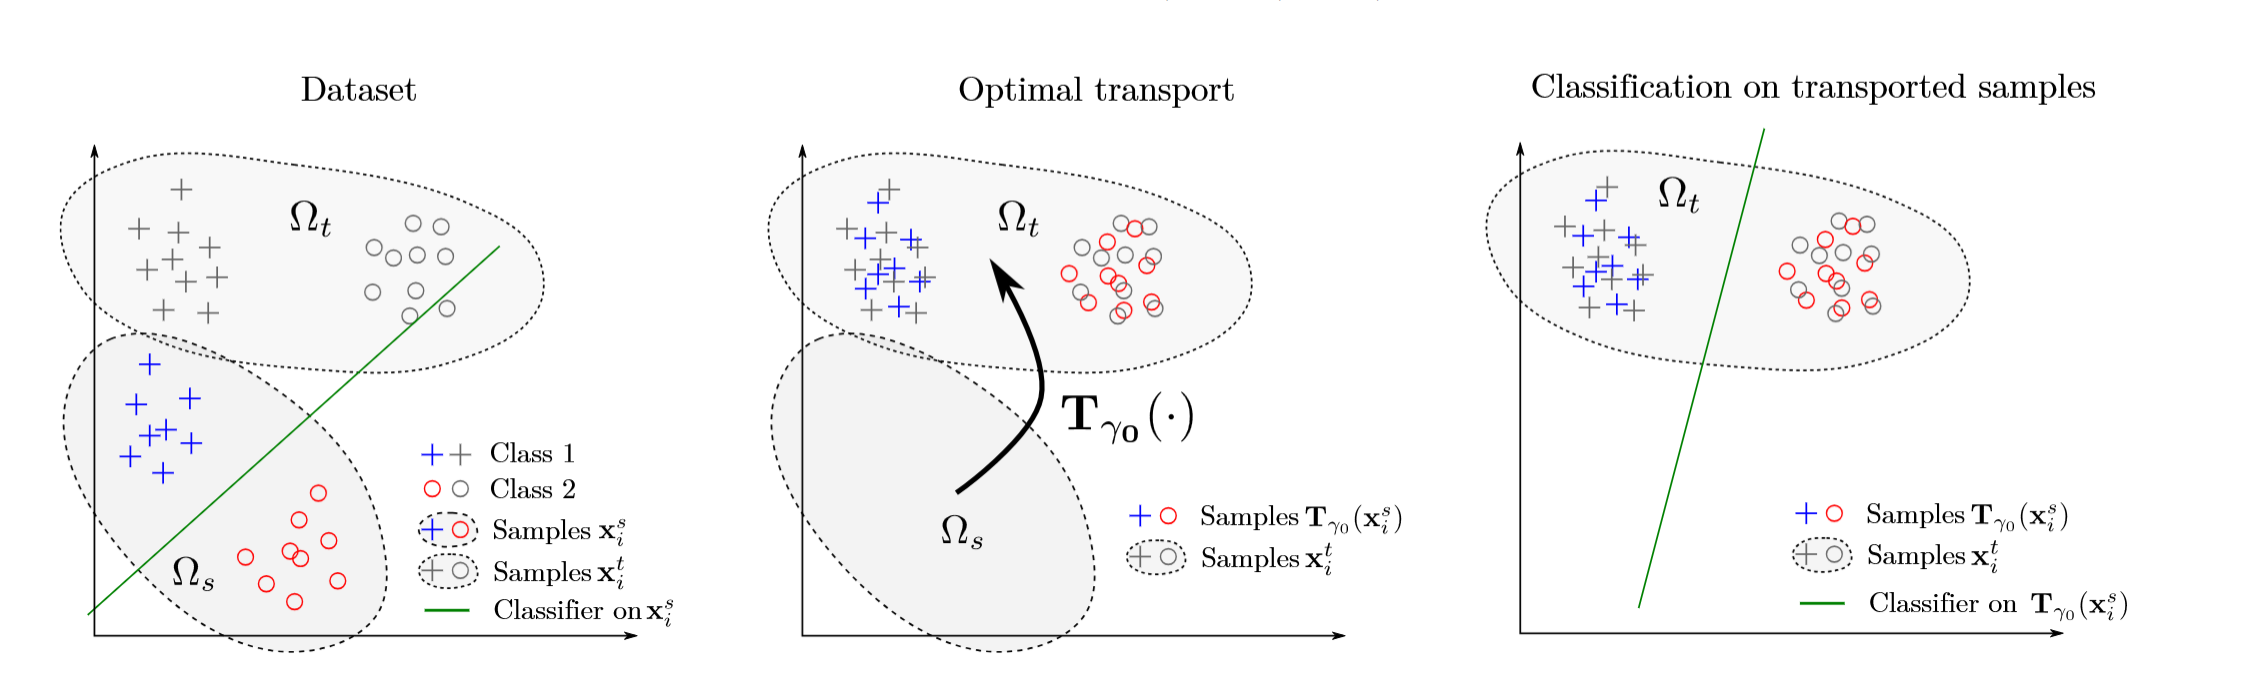
\includegraphics[width=0.78\textwidth]{image.png}

    \vspace{0.04cm}
    {\scriptsize
    Nếu source và target bị lệch nhau, classifier học trên source có thể không hợp với target.
    OT ``kéo'' source samples gần target hơn nhưng vẫn giữ label, rồi train classifier trên dữ liệu đã được kéo sang \cite{courty2017optimal}.}
\end{frame}

\section{Kết luận}

\begin{frame}{Takeaways}
    \begin{itemize}
        \item Discrete OT có thể nhìn như bài toán vận tải: supply, demand, cost, và plan $P$.
        \item Least Cost Method tạo nghiệm ban đầu nhanh nhưng chưa chắc tối ưu.
        \item MODI/u-v kiểm tra reduced cost để cải thiện nghiệm.
        \item Bảng transportation cũng có thể nhìn như bipartite graph/min-cost flow.
        \item Sinkhorn là phần mở rộng hiện đại: xấp xỉ nhanh, mềm hơn, hợp với ML.
    \end{itemize}
\end{frame}

\begin{frame}[allowframebreaks]{References}
    \bibliographystyle{ieeetr}
    \bibliography{references}
\end{frame}

\end{document}
